\documentclass{beamer}


\usepackage{cmap}
\usepackage[utf8]{inputenc}
\usepackage[T1]{fontenc}
\usepackage[english, russian]{babel}
\usepackage{cite}

\usepackage{graphicx}
\usepackage{amsmath}        % extensions for typesetting of math
\usepackage{amsfonts}       % math fonts
\usepackage{amsthm}         % theorems, definitions, etc.
\usepackage{amssymb}
\usepackage{subcaption}

\usepackage{adjustbox}
\usepackage{wrapfig}

%\usepackage{fancyvrb}       % improved verbatim environment
 %\usepackage{subfig}

%\bibliographystyle{iopart-num}
%\usepackage{iopams}
%\newcommand{\REVTeX}{REV\TeX}
%\usepackage{bm}
\usepackage{cleveref} 
\usepackage{tikz}


\graphicspath{ {C:/Users/Admin/Documents/Github/ProjectMagnet/Расчёты .ipynb/Images/} }


\title{Magnetic and Geometric Properties of the Ising Model on Lattice Random Walks}

\author{Ilya Pchelintsev\\
Scientific Adviser: Burovsky Evgeny Andreevich\\
The Department of Applied Mathmatics\\
National Research University "Higher School of Economics"\\
The Moscow Institute of Electronics and Mathematics\\
Moscow, Russia\\
iipchelintsev@edu.hse.ru}
\date{22nd of March, 2023}

\usetheme{Madrid}

\begin{document}

\begin{frame}
\titlepage
\end{frame}

\begin{frame}
\frametitle{Table of contents}
\tableofcontents
\end{frame}

\section{Introduction}

\begin{frame}{Ising-ISAW model}
\begin{itemize}
\item Linear self-avoiding conformation (\textbf{SAW}-models)
\item Spin subsistem inside of the monomers (regular \textbf{Ising model})
\item Close-range interaction \eqref{H_Ising_ISAW}
\item Tricriticality of the phase transition point \cite{Gennes1979}
\end{itemize}

\begin{figure}
\begin{subfigure}{0.35\textwidth}
\centering
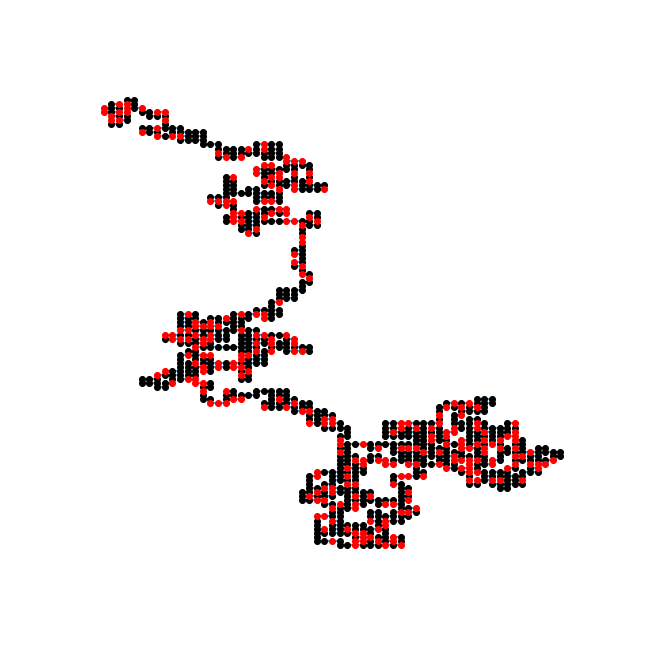
\includegraphics[width=\textwidth]{Globule_extented.png}
\end{subfigure}
\hfill
\begin{subfigure}{0.35\textwidth}
\centering
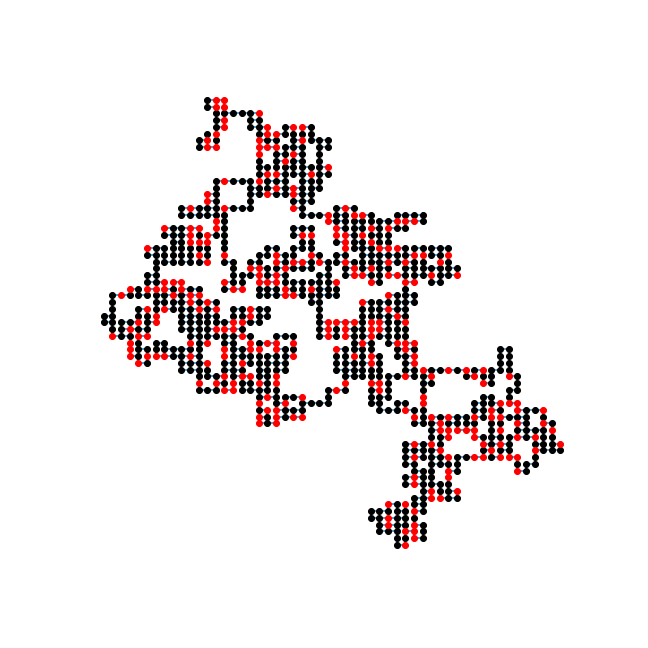
\includegraphics[width=\textwidth]{Globule_swollen.png}
\end{subfigure}
\begin{equation}\label{H_Ising_ISAW}
  H_{u, N, \{\sigma\}} = - \sum_{\langle i,j \rangle} J  \sigma_{i}  \sigma_{j},\ \ i,j \in u,\ |u| = N
\end{equation}
\end{figure}



\end{frame}

\begin{frame}{Universality of critical properties of the regular Ising model}

\begin{figure}
\centering
\begin{subfigure}{0.45\textwidth}
\begin{equation}\label{H_Ising_Rectan}
  H_{L, r, \{\sigma\}} = - \sum_{\langle i,j \rangle} J  \sigma_{i}  \sigma_{j}
\end{equation}
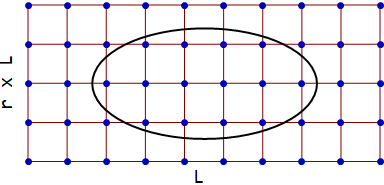
\includegraphics[width=\textwidth]{RectanGrid.png}
\caption{Example of the regular Ising model and its gyration ellipse}
\end{subfigure}
\hfill
\begin{subfigure}{0.45\textwidth}
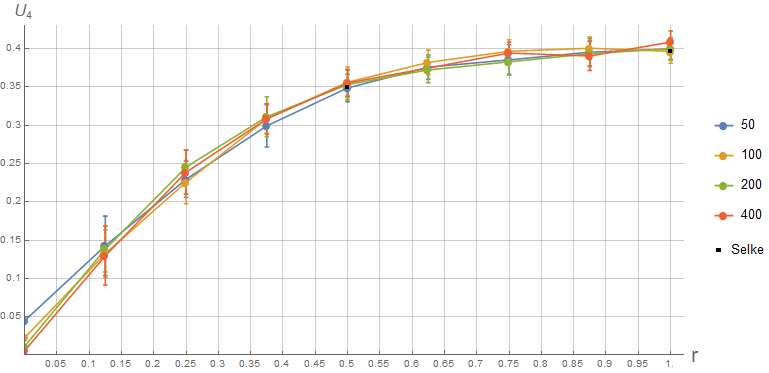
\includegraphics[width=\textwidth]{CumulantOBC.png}
\caption{Critical cumulant as a function of the lattice ratio \cite{Selke2006}}
\end{subfigure}
\end{figure}



\begin{alertblock}{Question №1}
Equal critical geometrical properties $\Rightarrow$ equal critical magnetic ones?
\end{alertblock}
\end{frame}

\begin{frame}{Lattice nearest-neighbors modifications}

\begin{figure}[t]
\centering
\begin{subfigure}{0.34\textwidth}
\centering
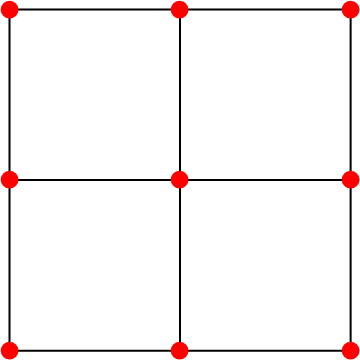
\includegraphics[width=0.7\textwidth]{SqLattice.png}
\end{subfigure}
\hfill
\begin{subfigure}{0.34\textwidth}
\centering
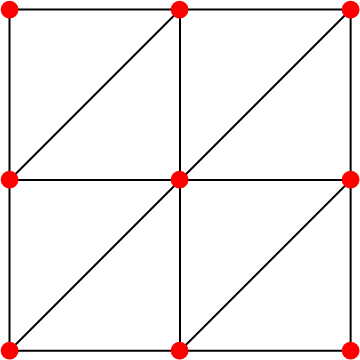
\includegraphics[width=0.7\textwidth]{TriLattice.png}
\end{subfigure}
\hfill
\begin{subfigure}{0.3\textwidth}
\centering
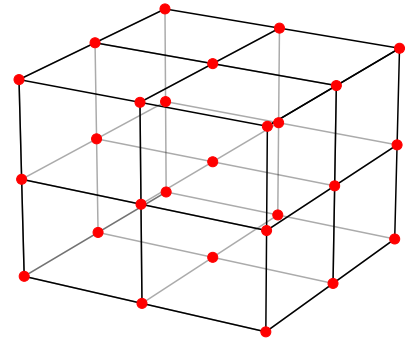
\includegraphics[width=1\textwidth]{Cubic_lattice_Cut.png}
\end{subfigure}

\begin{alertblock}{Question №2}
Universality of lattices with equal numbers of dimensions OR equal coordination numbers? 
\end{alertblock}
\end{figure}

\end{frame}

\begin{frame}{Observables}
Critical cumulant:
\begin{equation}
\label{eq:Cumulant}
U_{4} = 1 - \frac{\langle m^{4} \rangle}{3 \langle m^{2} \rangle^{2}}
\end{equation}
Gyration tensor of SAW-system \cite{Caracciolo2011}:
\begin{equation}\label{eq:Ten_G1}
    Q_{N,\alpha\beta} = \frac{1}{N} \sum^{N}_{i=1}(w_{i,\alpha} - w_{c, \alpha})(w_{i,\beta} - w_{c, \beta})
\end{equation}
Aspect ratio of the SAW-system:
\begin{equation}
    r = \sqrt{\frac{\langle q_{1}\rangle_{N}}{\langle q_{2} \rangle_{N}}}
\end{equation}
Asphericity:
\begin{equation}
\label{eq:Asphericity}
    \mathcal{A} = \left\langle \frac{(q_{1} - q_{2})^{2}}{(q_{1} + q_{2})^{2}} \right\rangle_{N}
\end{equation}

\end{frame}

\section{Results}

\begin{frame}{Critical Asphericity}

\begin{figure}
\centering
\begin{subfigure}{0.45\textwidth}
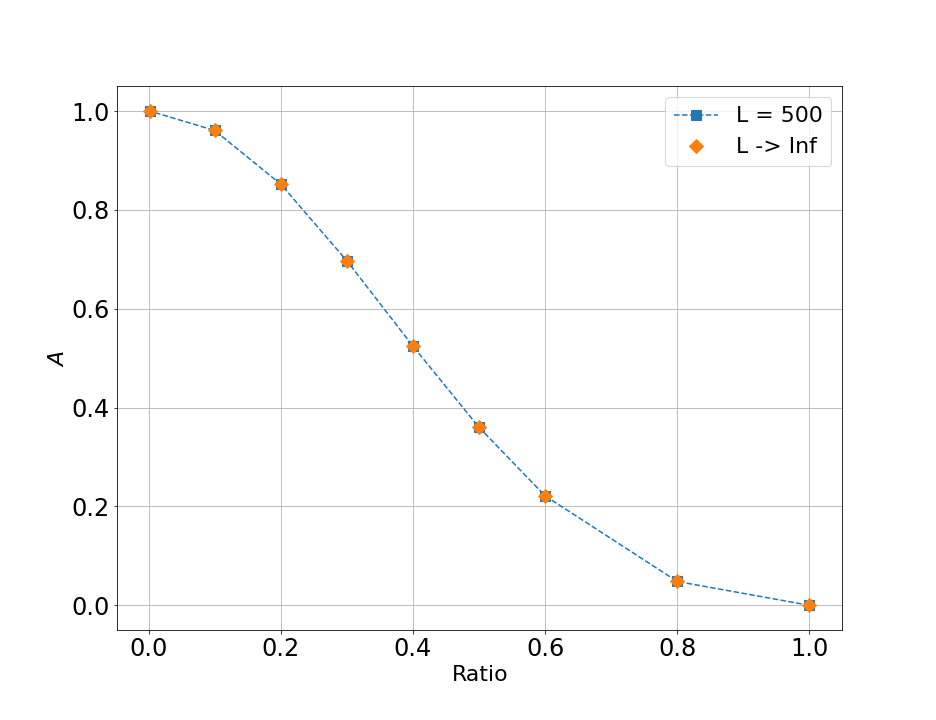
\includegraphics[width=\textwidth]{A_r.png}
\caption{Asphericity of the regular Ising as a function of the lattice ratio}
\end{subfigure}
\hfill
\begin{subfigure}{0.45\textwidth}
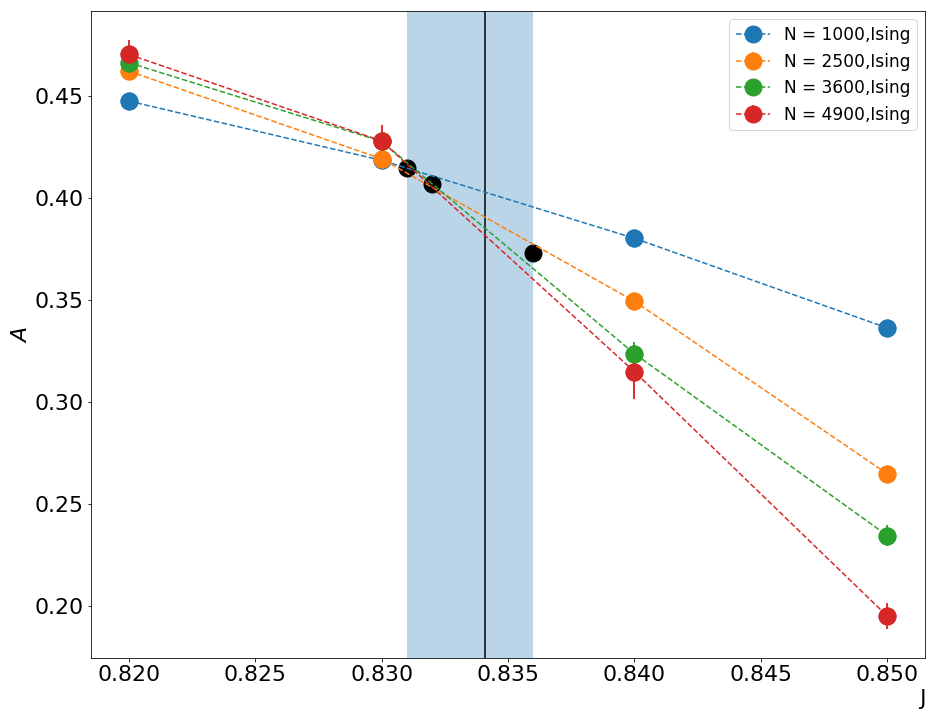
\includegraphics[width=\textwidth]{Ising_A_J_Close.png}
\caption{Asphericity of the Ising-ISAW as a function of J in the crit. region}
\end{subfigure}
\end{figure}


\begin{table}
\begin{tabular}{|c|c|c|}
    \hline
        Structure & lattice & $J_{c}$ \\ \hline
        SAW & Square & $0.8340(5)$\cite{faizullina2021critical} \\ \hline
        lattice & Rectangular & $\ln{(1 + \sqrt{2}) / 2}$\cite{Onsager}\\ \hline
\end{tabular}
\end{table}
\end{frame}

\begin{frame}{Results}

\begin{table}
\begin{tabular}{|c|c|c|c|}
        \hline
         \multicolumn{4}{|c|}{Ising-ISAW}  \\ \hline
         J & $\mathcal{A}$ & r & $U_{4}\  Rectangular$ \\ \hline
         0.831 & 0.415 & 0.465 & $0.338 \pm 0.006$\\ \hline
         0.832 & 0.4072 & 0.47 & $0.343 \pm 0.006$\\ \hline
         0.836 & 0.373 & 0.492 & $0.349 \pm 0.006$\\ \hline
\end{tabular}
\end{table}

\begin{block}{Result}
As for Ising-ISAW $U_4 = 0.308(8)$, critical cumulant showed \alert{complete mismatch}.
\end{block}

\end{frame}


\begin{frame}{Bulks of the Square lattice}
\begin{wrapfigure}{r}{0.2\textwidth}
    \centering
    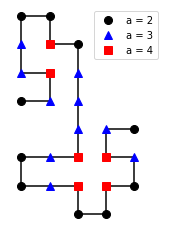
\includegraphics[width=0.2\textwidth]{count.png}
    \label{fig:example_bulk}
\end{wrapfigure}
Monomers according to the number of interactions:
\begin{itemize}
\item 2 neighbors - 1D-chains
\item 3 neighbors - boundaries of the cluster
\item 4 neighbors - core of the cluster
\end{itemize}
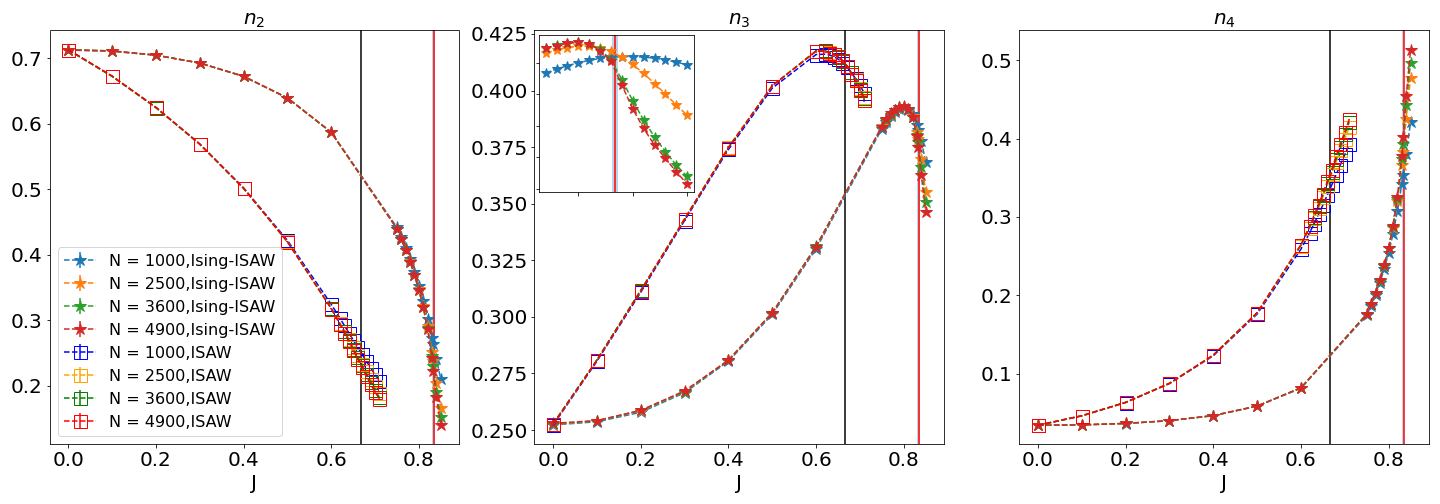
\includegraphics[width=0.8\textwidth]{bulk2-4_inset.png}
\end{frame}

\begin{frame}{Bulk results}
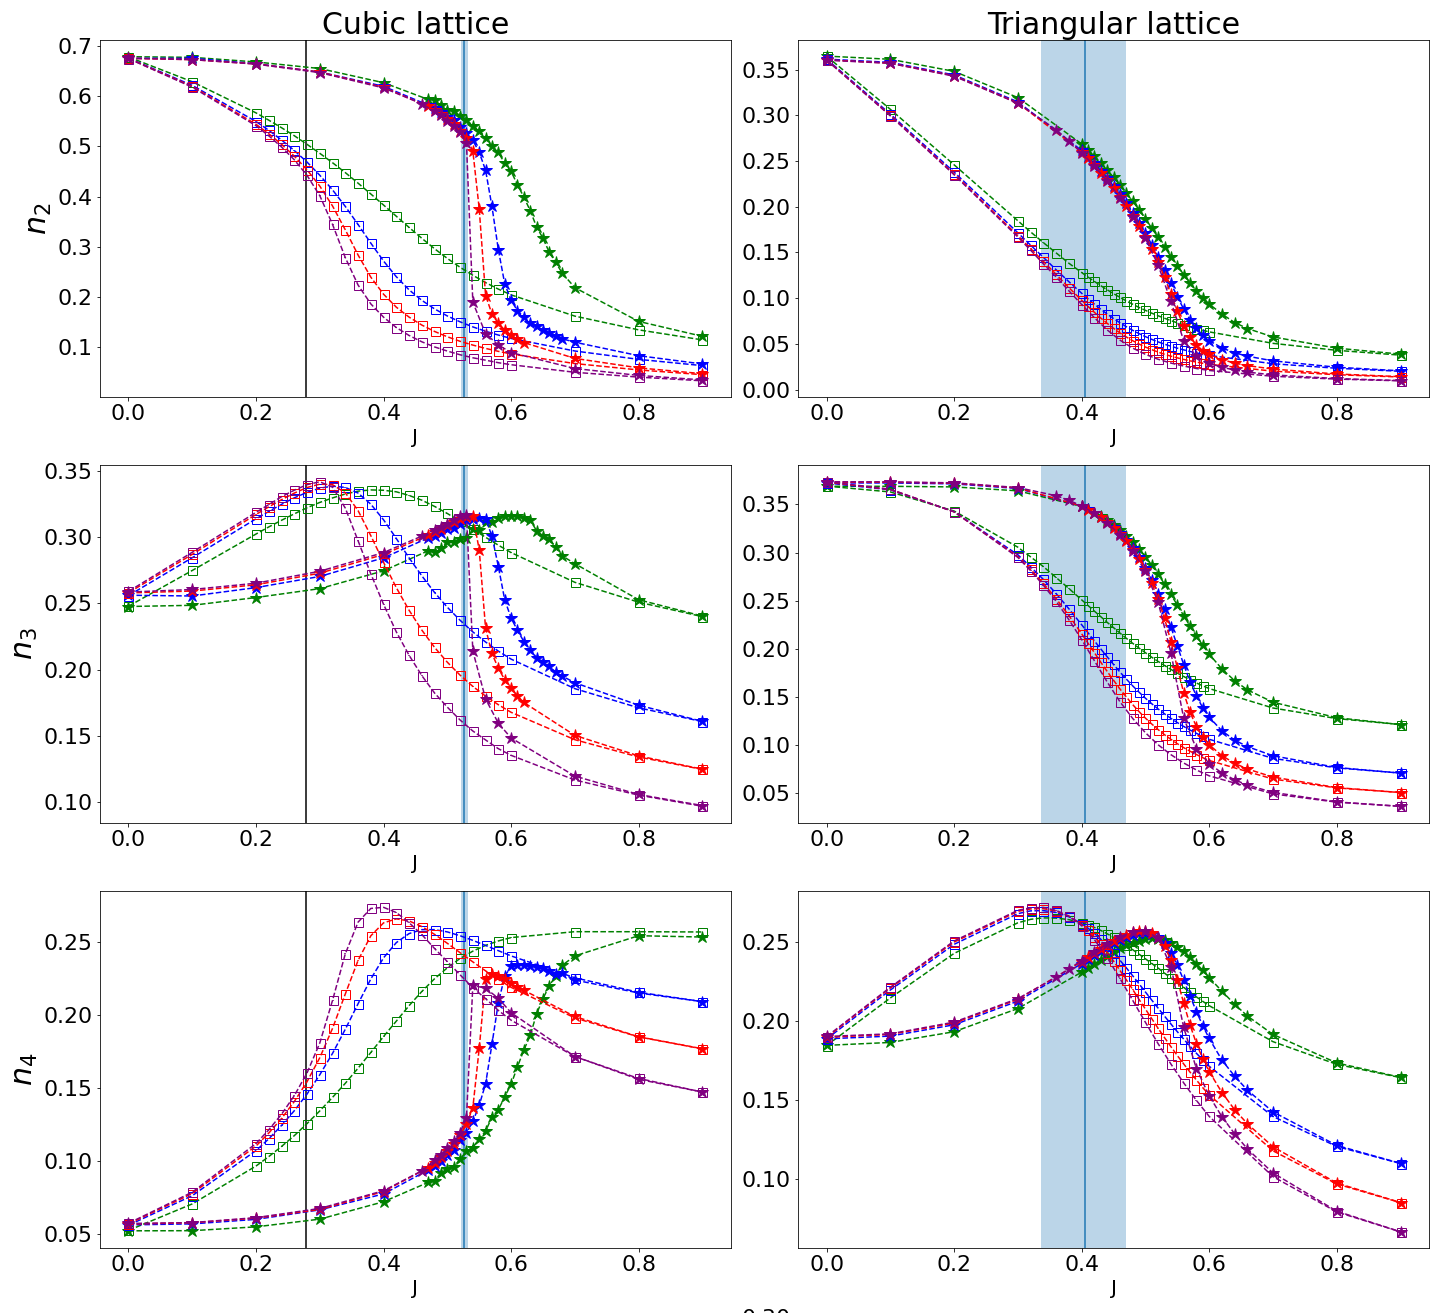
\includegraphics[width=0.45\textwidth]{Ising_vs_ISAW_2-4.png}
\hfill
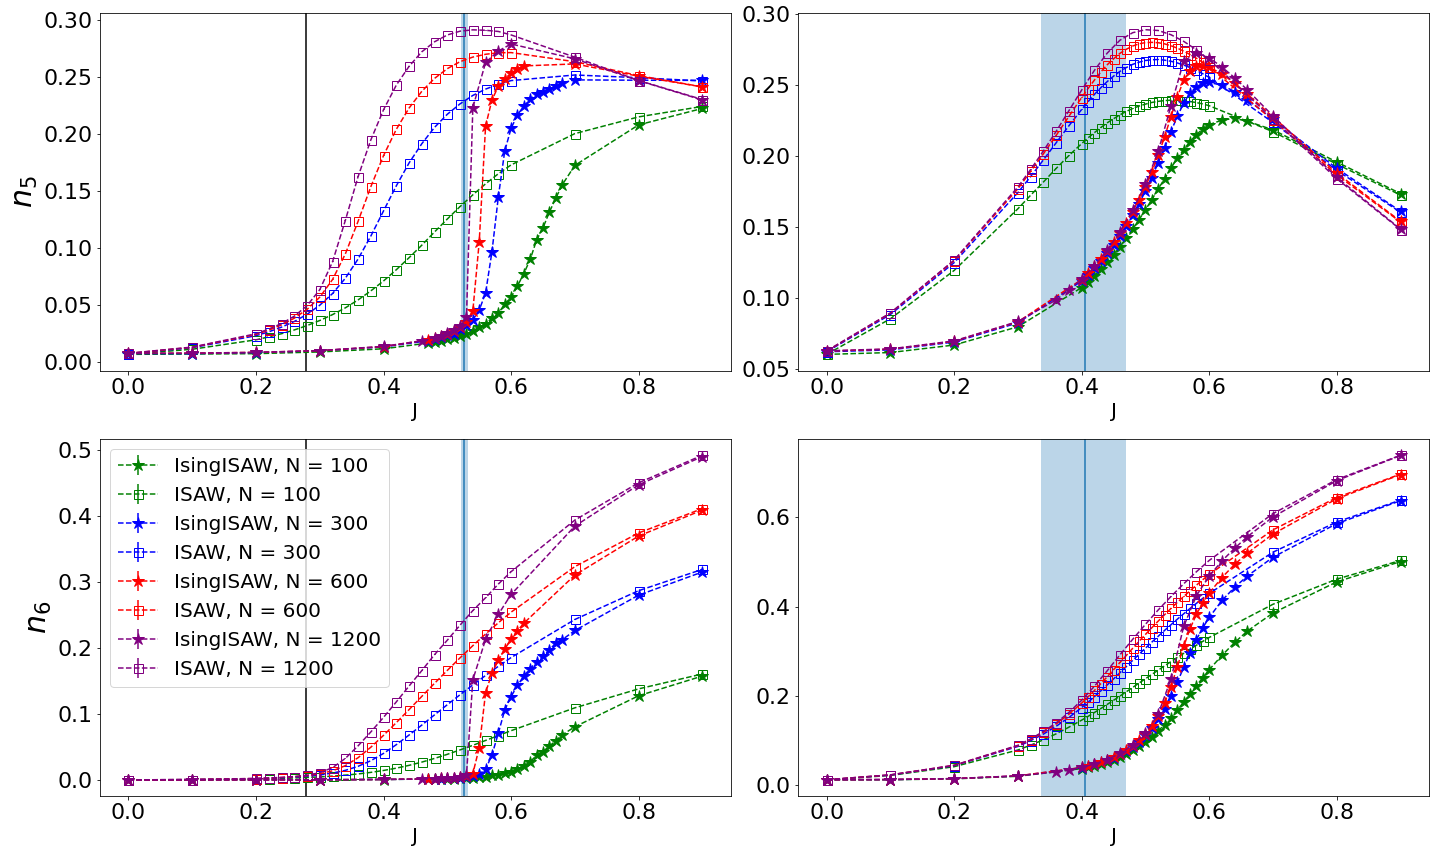
\includegraphics[width=0.45\textwidth]{Ising_vs_ISAW_5-6.png}
\begin{itemize}
\item First order transition was determined in cubic Ising-ISAW
\item Continious transition in triangular Ising-ISAW
\item Clear depiction of the chain consolidation
\end{itemize}

\end{frame}

\section{Future work}

\begin{frame}{Anticipated results}
\begin{columns}[t]
    \begin{column}{.45\textwidth}
      \adjincludegraphics[width=\textwidth, valign=t]{n23_linear.png}
    \end{column}
    \begin{column}{.45\textwidth}
	\alert{J=0 case research}:
      \begin{itemize}
        \item fractions scaling nature as functions of the chain length?  
        \item comparability of the lattice modifications
      \end{itemize}
    \end{column}
  \end{columns}
\end{frame}

\begin{frame}{References}

\bibliographystyle{IEEEtran}
\bibliography{bibliography}

\end{frame}

\begin{frame}

\begin{center}

\textit{ \LARGE Thanks for watching!}
\end{center}

\end{frame}

\end{document}